\documentclass[11pt]{article}

\usepackage{sectsty}
\usepackage{graphicx}
\usepackage{hyperref}
\usepackage{makecell}
\usepackage{listings}
\hypersetup{
    colorlinks=true,
    linkcolor=blue,
    filecolor=magenta,      
    urlcolor=cyan,
    }
\lstset{
    basicstyle=\ttfamily,
    columns=fullflexible,
    frame=single,
    breaklines=true,
    postbreak=\mbox{\textcolor{red}{$\hookrightarrow$}\space},
    }


\topmargin=-0.45in
\evensidemargin=0in
\oddsidemargin=0in
\textwidth=6.5in
\textheight=9.0in
\headsep=0.25in

\title{Algorithms for massive datasets project report \\ \vspace{10px} \large Market basket analysis}

\author{ Mattia Paravisi - 08395A }
\date{\today}

\begin{document}
\maketitle
\begin{center}
    \vfill
            
    I/We declare that this material, which I/We now submit for assessment, is entirely my/our own work and has not been taken from the work of others, save and to the extent that such work has been cited and acknowledged within the text of my/our work. I/We understand that plagiarism, collusion, and copying are grave and serious offences in the university and accept the penalties that would be imposed should I engage in plagiarism, collusion or copying. This assignment, or any part of it, has not been previously submitted by me/us or any other person for assessment on this or any other course of study
         
    \vspace{0.8cm}
\end{center}
\pagebreak

\pagebreak

%--Paper--


\section{Introduction}
\label{introduction}

This report includes the mental process I have followed during the development of the project, the code explanation, and some personal considerations. I chose to focus on market basket analysis for this project. The goal of this track is to implement a system from scratch that can find frequent itemsets, also known as market-basket analysis. In this context, the text field is considered as baskets and words, or other shingles, are treated as items. I have implemented the \textbf{Apriori algorithm} from scratch.

I decided to write the code for the Apriori algorithm because it serves as the baseline for some of the other algorithms covered in the lectures, such as SON and PCY. I believe that a well-implemented Apriori algorithm will pave the way for good implementations of the other two algorithms as well.

In market basket analysis the objective is to discover frequent itemsets that appear in the processed baskets in order to gain knowledge about the studied process. By using this set, it is possible to create association rules that are of interest. For this particular project, I utilized the "Yelp Dataset" which can be found \href{https://www.kaggle.com/datasets/yelp-dataset/yelp-dataset}{here}. Specifically, I focused on the review subset of the entire dataset, considering the "text" field and treating each JSON entry as a basket, with each word in the entry as an item.

The most recent access I made to the dataset was on June 7, 2023.
\section{Data Analysis and Pre-processing}
\label{data-analysis}

The dataset consists of approximately $6 \times 10^9$ reviews in JSON format, where each entry represents a user's review of a particular business. The schema of each entry is straightforward:

\begin{center}
    \resizebox{\textwidth}{!}{
    \begin{tabular}{|c|c|c|}
        \hline
        Attribute Name & Attribute Type & Attribute Meaning \\
        \hline
        business\_id & string & \makecell{This field represents the ID of the business being reviewed. \\ For example, a business\_id value could be "KU\_O5udG6zpxOg-VcAEodg".} \\
        \hline
        cool & long & \makecell{This field represents the number of "cool" reactions \\ given by other users to the current review.} \\
        \hline
        \dots & \dots & \dots \\
        \hline
        date & string & Date when the review was posted. \\
        \hline
        funny & long & Same as "cool". \\
        \hline
        text & string & \makecell{The actual text of the review. \textbf{This is the interesting field}.} \\
        \hline
    \end{tabular}
    }
\end{center}

As indicated in the table above, our focus is on analyzing the "text" attribute for all the reviews. This attribute contains the user's review of a business. As a first step I had to decide the type of items to consider: k-grams or words. Initially, I considered k-grams. To determine the value of $k$, I made a simple observation: the average length of a review in the dataset is 567 characters, and I assumed a character set cardinality of 27. My criteria for choosing $k$ was to have a low probability of finding each k-gram in each review. Therefore, by using $k = 4$, it is possible to create $27^4 >> 567$ k-grams. Although I could have used 4-grams, the median length of English words is 4, so I decided to directly use words as items to obtain more understandable results. Moreover, using k-grams would have increased the total number of items in a single review, adding complexity to the algorithm without significant benefits.

To tokenize the reviews, I initially considered using regular expressions but later opted for the NLTK package; it provides a pre-trained tokenizer for English text as well as a set of stopwords for the same language. The tokenization process is straightforward: I decided to convert each word to lowercase, remove numbers, and eliminate stopwords. Treating "As" and "as" as separate items would be redundant since they represent the same word. Including stopwords as items could lead to conceptually incorrect results. For example, it is true that "the" frequently appears with other words, but this is simply a characteristic of the language structure and is not significant in this context.

To proceed with the implementation, I extracted a sample of data from the entire dataset, selected only the "text" attribute, and applied the tokenization algorithm defined above to each review in the sample. I chose a small sample of approximately $7 \times 10^5$ reviews to ensure faster computation time. Since the project will not run in a distributed environment, I won't be able to leverage the distributed capabilities of Apache Spark.
\section{Apriori implementation}

I decided to implement the Apriori algorithm for the reasons I mentioned in chapter \ref{introduction}. 
\paragraph{Support functions}
I used only two support functions: the first one takes an item from the whole item set and gives as result an integer representation for that item, this function is useful to enhance main memory usage. Indeed each string, in Python, has a memory usage in bytes which \textbf{starts} from 40 bytes:

\begin{lstlisting}[language=Python]
    sys.getsizeof('')
    >> 40
\end{lstlisting}

for this reason encoding each string as an integer is convenient considered the fact that each integer occupies 32 bytes. The methods I wrote with this purpose of encoding/decoding are:

\begin{lstlisting}[language=Python]
    item_to_index = {}
    index_to_item = []

    def item_to_index_funct(item):
      if item not in item_to_index:
        item_to_index[item] = len(item_to_index.keys())
        index_to_item.append(item)
      return item_to_index[item]

    def index_to_item_funct(val):
      res = []
      if type(val) == int:
            return index_to_item[val]
      for sub_el in val:
            res.append(index_to_item[sub_el])
      return tuple(res)
\end{lstlisting}

the first method given an item checks if it is inside the dictionary item\_to\_index, if not it just creates a new entry which has as value the next integer with respect to the encoding of the previous item and as key the current item. After each insertion in the dictionary the method appends to an array the item, this is done to guarantee an inverse retrieval in time $O(1)$. The method index\_to\_item\_funct just access to the array using the given index.

For example, lets suppose that currently we have $n$ elements in the dictionary $x_0, \dots, x_n$. The dictionary's key-value couples are:
$$
(x_0,0),(x_1,1),\dots,(x_n,n)
$$
and the corresponding array is:
$$
[x_0,x_1,\dots,x_n]
$$
when the element $x_{n+1}$ arrives, in the dictionary will be created the tuple $(x_{n+1}, n+1)$ and $x_{n+1}$ will be appended to the array:
$$
(x_0,0),(x_1,1),\dots,(x_n,n),(x_{n+1},n+1)
$$
$$
[x_0,x_1,\dots,x_n,x_{n+1}]
$$
in this way, given a generic index $k$ to the second function the retrieval of $x_k$ is efficient.

\paragraph{Data pre-processing} Assumed that the sample mentioned in chapter \ref{data-analysis} is given, using classical Python code, I have applied the token to index method to each of the basket in the sample:
\begin{lstlisting}[language=Python]
  collected_data = [[item_to_index_funct(token) for token in review] for review in collected_data]
\end{lstlisting}
for each review in the sample I just apply the function mentioned above to all the tokens. The result of this operation is a list of lists of integers:
$$
[[0,11,3,\dots],[4,12,0,\dots],\dots]
$$
in each sub-list a single integer is the encoding for a specific word, each sub-list is the encoding for a single review.

\paragraph{Apriori} I decided to write just one function and exploit Spark's operations devoted to distributed computation to implement Apriori algorithm. It is mainly composed by two pieces: the first one is used to find frequent singletons, the second creates and filters new candidates, the latter will be executed until we have no more candidates. Starting from the first block of code:
\begin{lstlisting}[language=Python]
frequent_tuples =     data \
  .flatMap(lambda token: token) \
  .map(lambda token : (token, 1)) \
  .reduceByKey(lambda token_a, token_b : token_a + token_b) \
  .filter(lambda token : token[1] > support)
frequent_elems = frequent_tuples.map(lambda token: token[0])
\end{lstlisting}
the operations are:
\begin{itemize}
  \item The \textit{flatMap} is used to get a list of single tokens starting from the complete list of reviews. For example, if I have data which is 
  $$
  [[1,2],[2,3]]
  $$
  after the \textit{flatMap} I will have a single list
  $$
  [1,2,2,3]
  $$
  it is easy to apply a count pattern on those elements to get the frequency of each item.
  \item To apply the count pattern I had to \textit{map} all the elements in
  $$
  (key,1)
  $$
  the idea is to \textit{reduceByKey} summing by the value. This operation allows to obtain the absolute frequencies for the $key$. In the previous example, after the mapping, the list will be:
  $$
  [(1,1),(2,1),(2,1),(3,1)]
  $$
  \item \textit{reduceByKey} allows to sum the values and get the absolute frequece of each item
  $$
  [(1,1),(2,2),(3,1)]
  $$
  \item \textit{filter} just removes the items which frequence is not above the threshold we passed to the algorithm.
\end{itemize}

The second piece of my implementation does exactly the same thing but it is splitted in two sub cases depending on the fact that we are creating k-tuples with $k=2$ or $k>2$; this is due to how Python itertools module manage combinations with $k=1$ (when $k=2$ I am interested in each sub-tuple with $k=1$ in the couple). Here I will just describe one of the two sub parts. Lets consider for example the first one:
\begin{lstlisting}
if k == 2:

  data = spark.sparkContext.parallelize(data \
    .map(lambda indexed_element: [el[0] for el in combinations(indexed_element, k-1) if el[0] in collected_freq_elems.value])\
    .filter(lambda x: len(x) > k).collect())

  frequent_k_tuples = data \
    .flatMap(lambda indexed_element: [el for el in combinations(indexed_element, k) if set(el).issubset(set(collected_freq_elems.value))]) \
    .map(lambda token : (token, 1)) \
    .reduceByKey(lambda token_a, token_b : token_a + token_b) \
    .filter(lambda token : token[1] > support)
\end{lstlisting}

In the first assignment, into the parallelize method:
\begin{itemize}
  \item \textit{data} is the whole collected dataset.
  \item \textit{map} takes each review in data, for each review creates the combinations with cardinality 1,($k-1$ in this particular case is 1) and keeps the element only if it was frequent.
  \item \textit{filter} takes only the new reviews which have a length greater than 1 because I will then create combinations of two elements, for this reason I need that each review has at least two elements. 
\end{itemize}

The idea of this reassignment of \textbf{data} is that i want to keep at each iterations only the tokens that were frequent at the step before: it useless to compute each time a new filter on the whole review; indeed if in a couple $(x,y)$ i have that for instance $x$ is not frequent, i can filter out from the review that element because each couples with $x$ will be discarded anyway.

In the second assignment:
\begin{itemize}
  \item \textit{data} is the filtered version of the initial dataset.
  \item \textit{flatMap} allows me to create the combinations with cardinality 2.
  \item \textit{map} creates the couples for the count pattern.
  \item \textit{reduceByKey} allows to count the frequency of each couple.
  \item \textit{filter} allows to keep only the elements which frequency is greater than the support.
\end{itemize}

I continue to apply this steps until the set of frequent items is empty.
\section{Experiments}

I decided to do perform two kinds of experiments: the first is devoted to find relationships between the number of frequent items the algorithm is able to find, the threshold and the execution time. My thesis was: the higher the threshold, the faster the algorithm will finish but the less number of results will be found. This is not surprising at all: if we increment the threshold we are asking to a generic k-tuple of elements, in order to be considered frequent, to appear a number of times which is higher and higher. With this experiment I wanted to check how fast this reduction would happen, i was expecting a gradual lowering of the frequent set cardinality, the result denies me:
\begin{figure}[h]
    \caption{Relationships between execution time, support threshold, number of frequent items found}
    \centering
    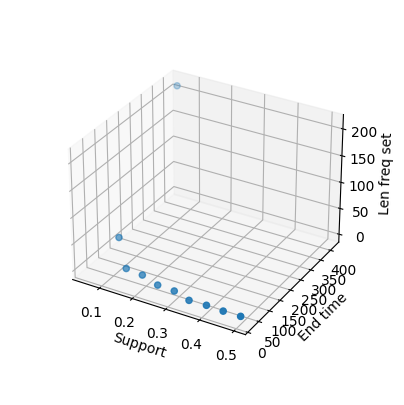
\includegraphics[width=0.5\textwidth]{project_report_src/project_report_images/support_end-time_len-freq-set.png}
\end{figure}

when the threshold changes from the 5\% to the 10\% the number of frequent items decreases abruptly: 211 with the first threshold and 48 with the latter.This result means that there a lot of k-tuples which are somehow borderline: they are frequent with the first threshold but the number of occurencies is very close to the threshold itself. This may be related to the fact that the structure of language is very complex, for example the presence of synonyms can lead to this result. In fact, there are a lot of words which can be used instead of "good", for example, and those words are used by a smaller number of reviewers, for this reason the itemsets with "delicious" (for example) as item are took into consideration with $threshold = 0.05$ but not with $threshold = 0.10$ . As I suspected the execution time got lower as the threshold increased, this is a natural behaviour given by the structure of the algorithm: when the threshold increases it is able to filter out more elements and this filtering allows to create less k-tuples, for this reason the overall computational time get lower.

The second experiment had the aim of checking the scaling for the algorithm. I runned the algorithm with an incremental number of rows from $1 \cdot 10^5$ to $7 \cdot 10^5$, with $1 \cdot 10^6$ and with $1.5 \cdot 10^6$ and i checked only the execution time:
\begin{figure}[h]
    \caption{Relationships between execution time and number of rows}
    \centering
    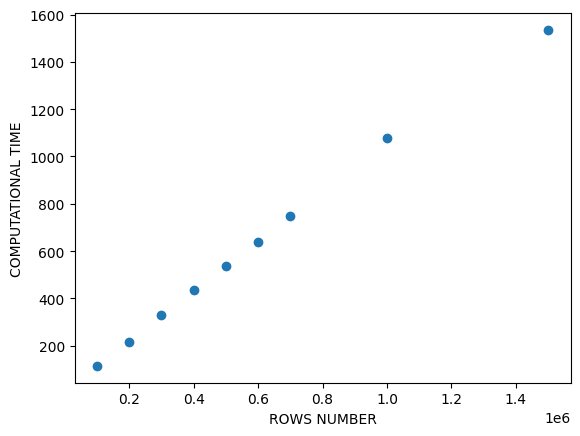
\includegraphics[width=0.5\textwidth]{project_report_src/project_report_images/scaling.png}
\end{figure}
the growth is linear, this is a good signal for the algorithm robustness. 

%--/Paper--

\end{document}
